% ####### Compiler     : pdflatex
% ####### Bibliography : bibtex

%% add option 'print' for print version
%% leave blank or add option 'online' for online version
\documentclass[print]{../class/csthesis}

% ####################### User Packages #######################
\usepackage[export]{adjustbox}
\usepackage{lipsum}

% ################# Specify path for graphics #################
\graphicspath{{figs/}{../figs/}}

% ############# Command for algorithm environment #############
\algnewcommand\algorithmicinput{\textbf{INPUT:}}
\algnewcommand\INPUT{\item[\algorithmicinput]}
\algnewcommand\algorithmicoutput{\textbf{OUTPUT:}}
\algnewcommand\OUTPUT{\item[\algorithmicoutput]}

\algblockdefx{FOR}{ENDFOR}[1]%
{\textbf{for }#1 \textbf{do}}%
{\textbf{end for}}

% ###################### Where condition ######################
\newenvironment{conditions}[1][where:]
{#1
	\begin{tabular}[t]{>{}l<{} @{} >{${}}c<{{}$} @{} >{\raggedright\arraybackslash}p{0.8\textwidth}}}
	{\end{tabular}\par\vspace{\belowdisplayskip}}

% ############## Define my custom theorem style ###############
\newtheoremstyle{mystyle}% name of the style to be used
	{3pt}% measure of space to leave above the theorem. E.g.: 3pt
	{3pt}% measure of space to leave below the theorem. E.g.: 3pt
	{\normalfont}% name of font to use in the body of the theorem
	{\parindent}% measure of space to indent
	{\bf}% name of head font
	{}% punctuation between head and body
	{1em}% space after theorem head; " " = normal interword space
	{}% Theorem head spec (can be left empty, meaning ‘normal’)

% Command for use of the defined theorem style
\theoremstyle{mystyle}

% Define theorem
% Usage: \newtheorem{theorem}{Theorem}[chapter]
\newtheorem{example}{Example}

% ## Show the equation on multiple pages when it is too long ##
\allowdisplaybreaks 

% #############################################################
\newenvironment{prosNcons}[1]{
\indent \textbf{#1}\\ \indent
}

% ############### Specify words for hyphenation ###############
\hyphenation{SE-COMPAX speci-fies preecha-veerakul}

%% Print bibilography in subfiles when subfiles.tex is separately compiled
\newboolean{printBibInSubfiles}
\setboolean{printBibInSubfiles}{true} 
\def\bib{\ifthenelse{\boolean{printBibInSubfiles}}
	{\bibliographystyle{../main/IEEEtran}
		\bibliography{../main/references}}
	{}
}

\begin{document}
%% Not print bibilography in subfiles when thesis.tex is compiled
\setboolean{printBibInSubfiles}{false}

% ################## Preliminary Information ##################
% Specify crest
%\crest{
\includegraphics[width=2.36cm, height=3.43cm]{logo/psubw.png}}

% Specify page number style for inner pages
% Usage: \frontPageStyle{<style>}
% Default: \frontPageStyle{Roman}
% Parameter: roman (i, ii, ...), Roman (I, II, ...)
\innerPageStyle{Roman}

% Title showing on cover page which probably contains multiple lines
% Author add \\ for a new line manually
% Usage: \titleCover{<value with \\ command}
\titleCover{HyBiX: Hybrid Encoding Bitmap Index for \\Efficient Space and Query Processing Time}

% Title showing on abstract page
% Title must not contain new line command ( \\ )
\title{HyBiX: Hybrid Encoding Bitmap Index for Efficient Space and Query Processing Time}

% Personal Information
% Usage: \authorInfo{<title>}{<firstname>}{<lastname>}{<student id}
\authorInfo{Mr.}{Naphat}{Keawpibal}{5710230025}

% Define degree
% Usage: \degree{<value>}
\degree{Doctor of Philosophy}

% Major program showing on cover page
% Major program probably contains multiple lines
% Use \\ for new line
\majorProgramCover{Computer Science \\(International Program)}

% MajorProgram without breakline
\majorProgram{Computer Science (International Program)}

% Define degree year showing on cover page
% Usage: \degreeyear{<year>}
\degreeyear{2018}

% Define: academic year showing on abstract page
% Usage: \academicyear{<year>}
\academicyear{2018}

% Define: study plan
% Usage: \studyplan{<value>}
% <value>: PhD1 and PhD2, case sensitive.
\studyplan{PhD2}

% Define: advisor name
% Usage: \majoradvisor{<name>}
\majoradvisor{Asst. Prof. Dr. Sirirut Vanichayobon}

% Define: coadvisor name
% Usage: \coadvisor{<name>}
\coadvisor{Asst. Prof. Dr. Ladda Preechaveerakul}


% ######################### Committee #########################
% Define: chairperson
% Usage: \chairperson{<name>}
\chairperson{Assoc. Prof. Dr. Ohm Sornil}
% Define: 1st committee, this is your advisor
% Usage: \committeeOne{<name>}
\committeeOne{Asst. Prof. Dr. Sirirut Vanichayobon}
% Define: 2nd committee, this is your co-advisor if any
% Usage: \committeeTwo{<name>}
\committeeTwo{Asst. Prof. Dr. Ladda Preechaveerakul}
% Define: 3rd committee
% Usage: \committeeThree{<name>}
\committeeThree{Asst. Prof. Dr. Wiphada Wettayaprasit}
% Define: 4th committee, if any
% Usage: \committeeFour{<name>}
%\committeeFour{}

% Define: current dean of graduate school
% Usage: \deanOfGraduateSchool{<name>}
\deanOfGraduateSchool{Prof. Dr. Damrongsak  Faroongsarng}

% Create cover page
\begin{titlepage}
  	\maketitle
\end{titlepage}

% Create inner title page
\begin{innertitlepage}
  	\makeCSthesistitle
\end{innertitlepage}

% Create approval page
\begin{othertitlepage}
	\makeApprovalPage
\end{othertitlepage}

% Create declaration pages
\begin{othertitlepage}
	\makeDeclaration
\end{othertitlepage}

% For only thai students
% Add PDF file of thai abstract
% The thai abstract was created by Microsoft Word and exported as PDF file
% Note: Comment it if you are an international student
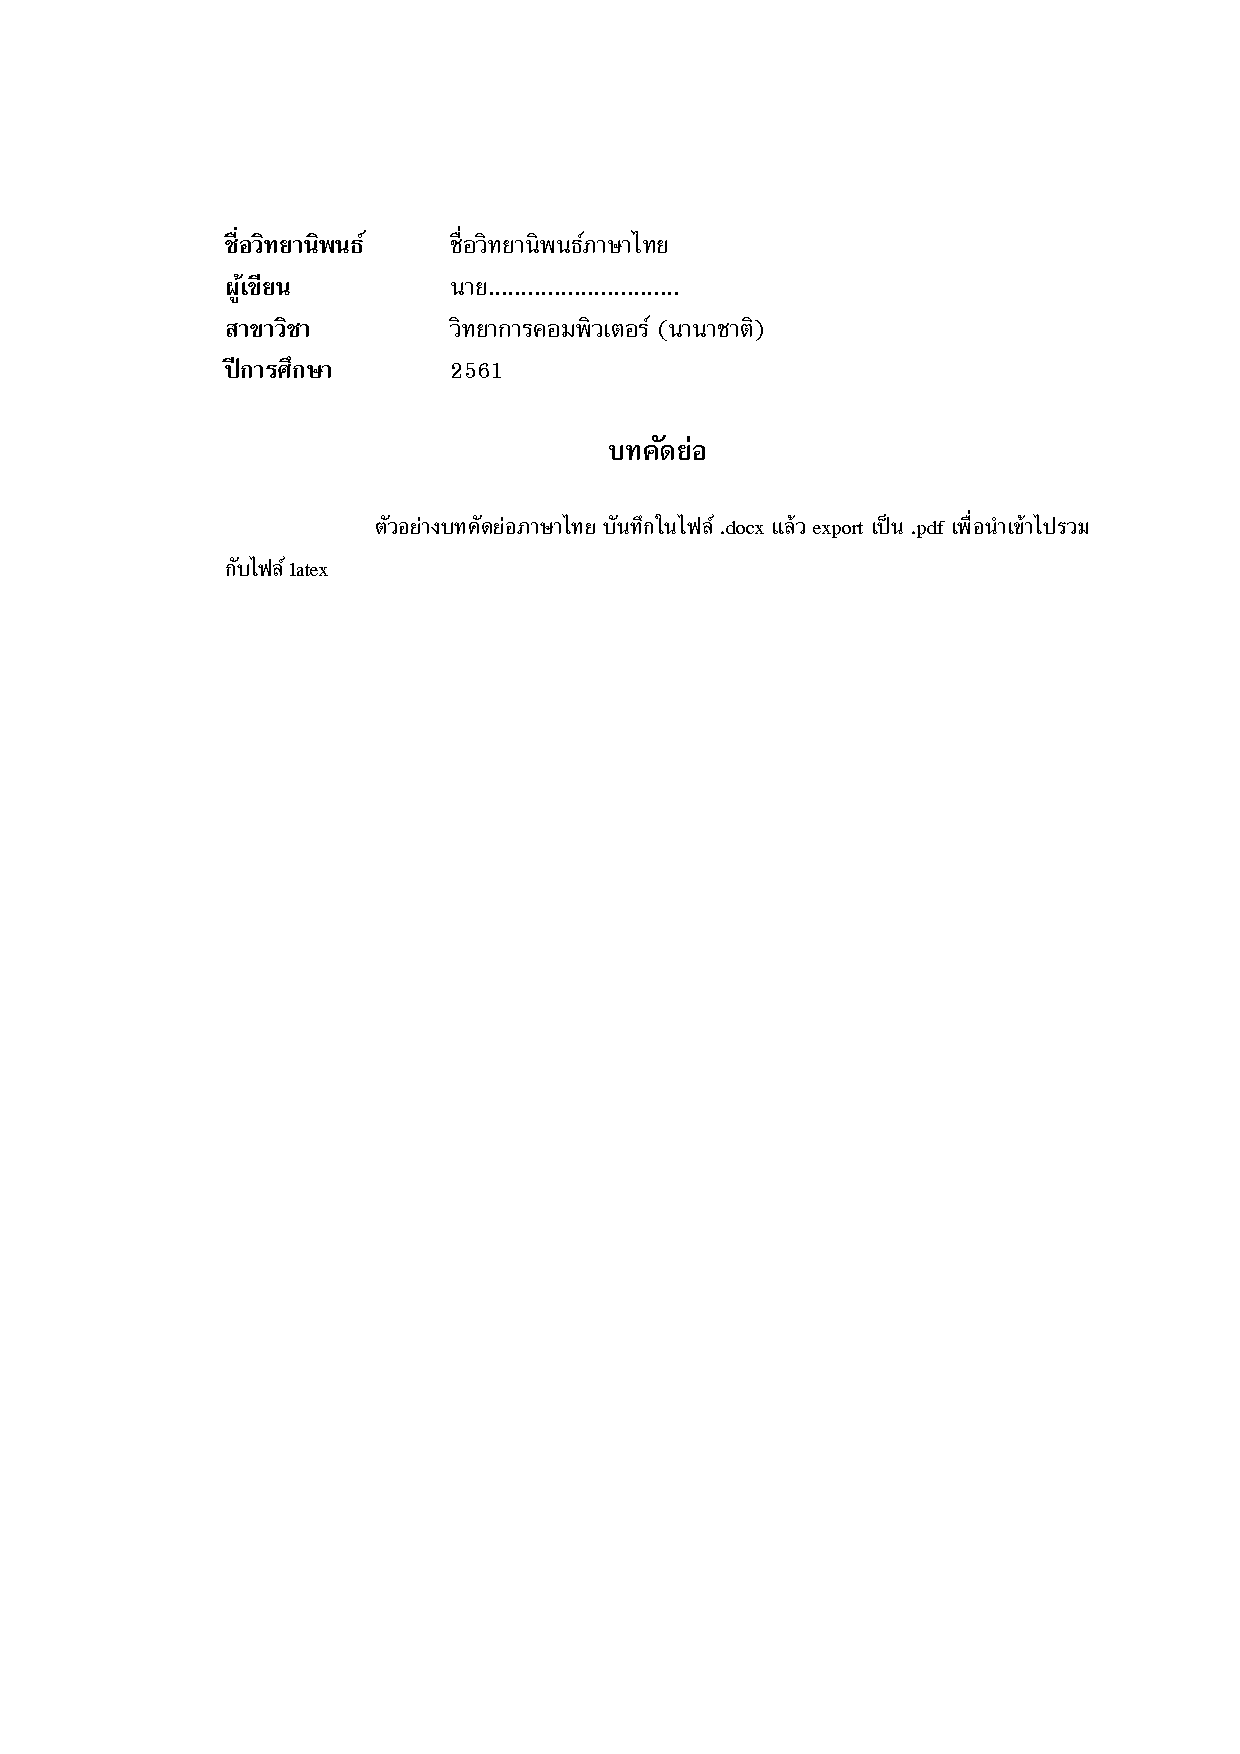
\includepdf[pages=-, pagecommand={\phantomsection\addcontentsline{toc}{chapter}{ABSTRACT (Thai)}}]{../abstract/abstractTH.pdf}

% Add english abstract page
\subfile{../abstract/abstractEN}

% Add acknowledgment page
\subfile{../acknowledgement/acknowledgement}

% ################## TOC, LOT, LOF, and LOA ###################
\CStableofcontents
\CSlistoftables
\CSlistoffigures
\CSlistofalgorithms

% Add "CHAPTER" before list of chapters in TOC
\addtocontents{toc}{\tocheading}

% ######################## Main Matter ########################
\mainmatter
\subfile{../chapter1/chapter1}
%\subfile{../chapter2/chapter2}
%\subfile{../chapter3/chapter3}
%\subfile{../chapter4/chapter4}
%\subfile{../chapter5/chapter5}
%\subfile{../chapter6/chapter6}

% ####################### Bibliography ########################
% Bibliography based on IEEE style
% Using bibliography file with extension .bib, e.g., references.bib
\begin{CSbib}
	\bibliographystyle{IEEEtran}
	\bibliography{references}
\end{CSbib}

% ######################## Appendices #########################
%\addtocontents{toc}{\protect\setcounter{tocdepth}{0}}
%\begin{appendices} % Using appendices environment for more functunality
%	\subfile{../appendix/appendix1}
%	%\subfile{../appendix/appendix2}
%\end{appendices}

% ########################## Vitae ############################
\subfile{../vitae/vitae}

\end{document}